\chapter{Bandwise Grayscale Reconstructions}
\label{appendix:bandwise_results}

\begin{figure}[h!]
    \centering
    \captionsetup[subfigure]{labelformat=empty}

    % ---------- Row 1 ----------
    \begin{subfigure}{0.48\textwidth}
        \centering
        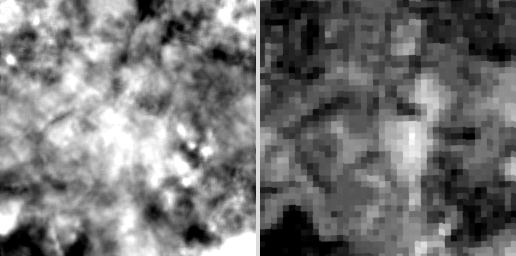
\includegraphics[width=\linewidth]{img/bands_gray/sample_000008_B01_panel.png}
        \caption{B1 (Aerosols, 443 nm)}
    \end{subfigure}\hfill
    \begin{subfigure}{0.48\textwidth}
        \centering
        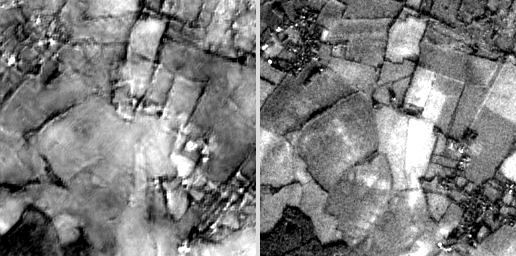
\includegraphics[width=\linewidth]{img/bands_gray/sample_000008_B02_panel.png}
        \caption{B2 (Blue, 490 nm)}
    \end{subfigure}

    % ---------- Row 2 ----------
    \vspace{0.5em}
    \begin{subfigure}{0.48\textwidth}
        \centering
        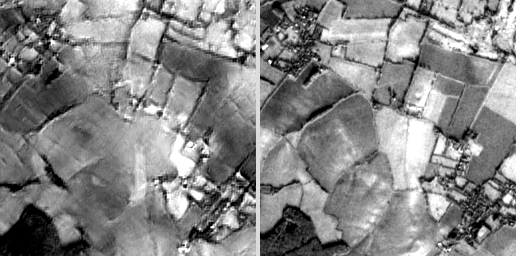
\includegraphics[width=\linewidth]{img/bands_gray/sample_000008_B03_panel.png}
        \caption{B3 (Green, 560 nm)}
    \end{subfigure}\hfill
    \begin{subfigure}{0.48\textwidth}
        \centering
        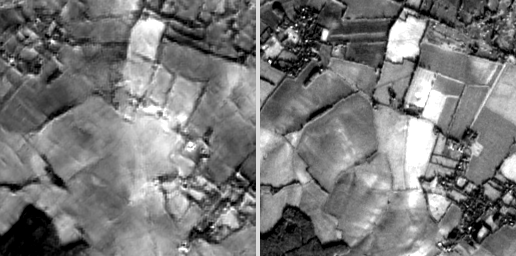
\includegraphics[width=\linewidth]{img/bands_gray/sample_000008_B04_panel.png}
        \caption{B4 (Red, 665 nm)}
    \end{subfigure}

    % ---------- Row 3 ----------
    \vspace{0.5em}
    \begin{subfigure}{0.48\textwidth}
        \centering
        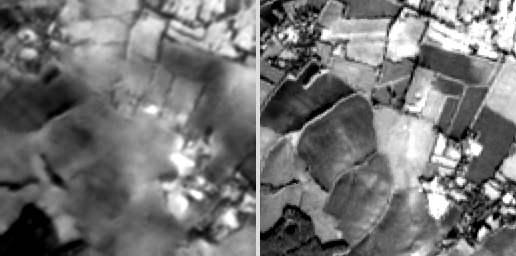
\includegraphics[width=\linewidth]{img/bands_gray/sample_000008_B05_panel.png}
        \caption{B5 (Red Edge, 705 nm)}
    \end{subfigure}\hfill
    \begin{subfigure}{0.48\textwidth}
        \centering
        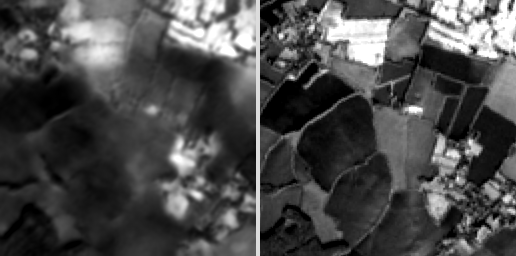
\includegraphics[width=\linewidth]{img/bands_gray/sample_000008_B06_panel.png}
        \caption{B6 (Red Edge, 740 nm)}
    \end{subfigure}

    \caption[Bandwise grayscale reconstructions (Bands 1–6)]%
    {Generated (left) and ground-truth (right) grayscale representations for Sentinel-2 Bands~1–6.}
    \label{fig:appendix_band_panels}
\end{figure}

\begin{figure}[p]
    \ContinuedFloat
    \centering
    \captionsetup[subfigure]{labelformat=empty}

    % ---------- Row 4 ----------
    \begin{subfigure}{0.48\textwidth}
        \centering
        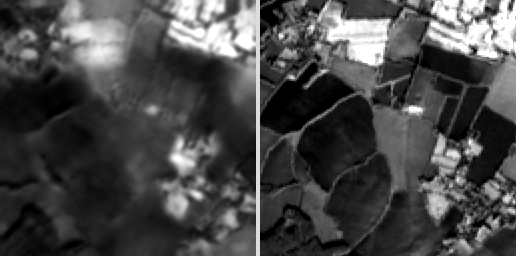
\includegraphics[width=\linewidth]{img/bands_gray/sample_000008_B07_panel.png}
        \caption{B7 (Red Edge, 783 nm)}
    \end{subfigure}\hfill
    \begin{subfigure}{0.48\textwidth}
        \centering
        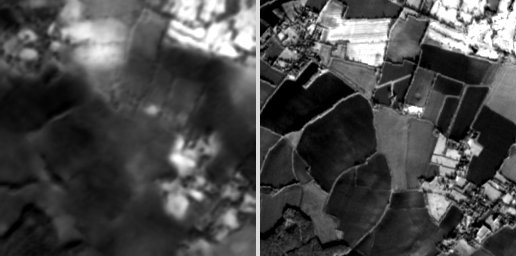
\includegraphics[width=\linewidth]{img/bands_gray/sample_000008_B08_panel.png}
        \caption{B8 (NIR, 842 nm)}
    \end{subfigure}

    % ---------- Row 5 ----------
    \vspace{0.5em}
    \begin{subfigure}{0.48\textwidth}
        \centering
        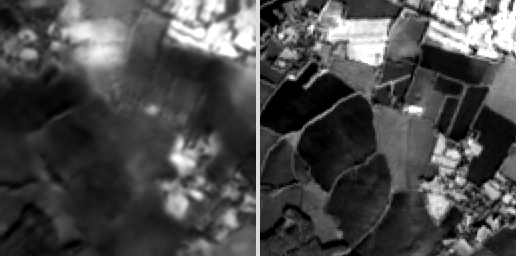
\includegraphics[width=\linewidth]{img/bands_gray/sample_000008_B09_panel.png}
        \caption{B8A (Red Edge, 865 nm)}
    \end{subfigure}\hfill
    \begin{subfigure}{0.48\textwidth}
        \centering
        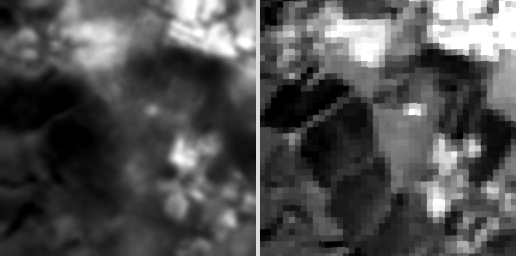
\includegraphics[width=\linewidth]{img/bands_gray/sample_000008_B10_panel.png}
        \caption{B9 (Water Vapour, 945 nm)}
    \end{subfigure}

    % ---------- Row 6 ----------
    \vspace{0.5em}
    \begin{subfigure}{0.48\textwidth}
        \centering
        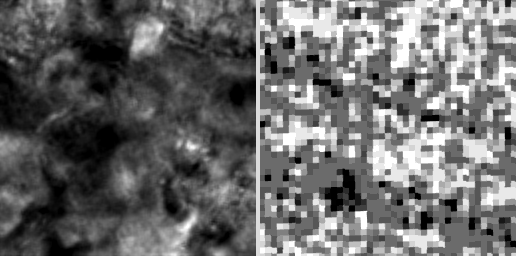
\includegraphics[width=\linewidth]{img/bands_gray/sample_000008_B11_panel.png}
        \caption{B10 (Cirrus, 1375 nm)}
    \end{subfigure}\hfill
    \begin{subfigure}{0.48\textwidth}
        \centering
        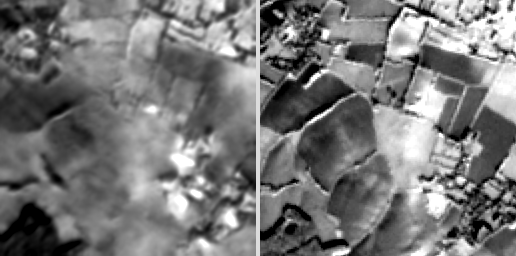
\includegraphics[width=\linewidth]{img/bands_gray/sample_000008_B12_panel.png}
        \caption{B11 (SWIR, 1610 nm)}
    \end{subfigure}

    % ---------- Row 7 ----------
    \vspace{0.5em}
    \begin{subfigure}{0.48\textwidth}
        \centering
        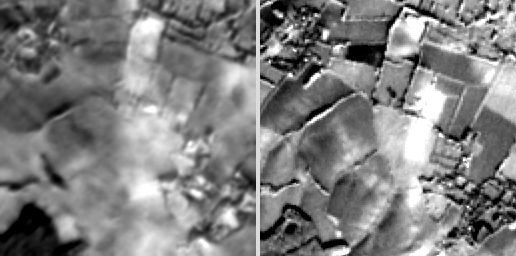
\includegraphics[width=\linewidth]{img/bands_gray/sample_000008_B13_panel.png}
        \caption{B12 (SWIR, 2190 nm)}
    \end{subfigure}

    \caption[Bandwise grayscale reconstructions (Bands 7–12)]%
    {Generated (left) and ground-truth (right) grayscale representations for Sentinel-2 Bands~7–12.}
\end{figure}


\chapter{Additional Quantitative Results}
\label{appendix:quantitative}
This appendix presents supplementary evaluation metrics and additional tables...

\chapter{Implementation Details}
\label{appendix:implementation}
Here, the complete model configuration and training hyperparameters are documented.

\chapter{Example Code Snippets}
\label{appendix:code}
The following excerpts show the main evaluation loop used in the experiments.
